\problemname{A Rational Sequence}

\noindent
An infinite full binary tree labeled by positive rational numbers is defined by:

\begin{itemize}
    \item The label of the root is \texttt{1/1}.
    \item The left child of label \texttt{p/q} is \texttt{p/(p+q)}.
    \item The right child of label \texttt{p/q} is \texttt{(p+q)/q}.
\end{itemize}

The top of the tree is shown in the following figure:

% insert image
\begin{figure}[!h]
    \begin{center}
        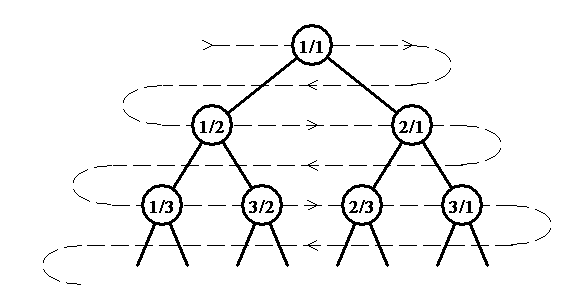
\includegraphics[]{f1.png} \\
    \end{center}
\end{figure}

A rational sequence is defined by doing a level order (breadth first)
traversal of the tree (indicated by the light dashed line).  So that:

\begin{verbatim}
F(1) = 1/1, F(2) = 1/2, F(3) = 2/1, F(4) = 1/3, F(5) = 3/2, F(6) = 2/3, ...
\end{verbatim}

Write a program which takes as input a rational number, \texttt{p/q}, in 
lowest terms and finds the next rational number in the 
sequence. That is, if  \texttt{F(n) = p/q}, then the result is \texttt{F(n+1)}.

\section*{Input}

The first line of input contains a single integer P, ($1 \le P \le 1000$),
which is the number of data sets that follow.  Each data set should be
processed identically and independently.

Each data set consists of a single line of input.  It contains the data
set number, $K$, which is then followed by a space, then the numerator of
the fraction, $p$, followed immediately by a forward slash (/), followed
immediately by the denominator of the fraction, $q$.  Both $p$ and $q$ will
be relatively prime and  $0 \le p, q \le 2,147,483,647$.

\section*{Output}

For each data set there is a single line of output.  It contains the
data set number, $K$, followed by a single space which is then followed
by the numerator of the fraction, followed immediately by a forward
slash (\texttt{/}) followed immediately by the denominator of the fraction.
Inputs will be chosen such that neither the numerator nor the denominator
will overflow a 32-bit integer.

